%%%%%%%%%%%%%%%%%%%%%%%%%%%%% -*- Mode: Latex -*- %%%%%%%%%%%%%%%%%%%%%%%%%%%%
%% 05-01-intro.tex -- Priority Ranked Software Inspection
%% Author          : Aaron A. Kagawa
%% Created On      : Mon Sep 23 11:52:28 2004
%% Last Modified By: Aaron Kagawa
%% Last Modified On: Tue Jul  5 20:09:40 2005
%% RCS: $Id$
%%%%%%%%%%%%%%%%%%%%%%%%%%%%%%%%%%%%%%%%%%%%%%%%%%%%%%%%%%%%%%%%%%%%%%%%%%%%%%
%%   Copyright (C) 2004 Aaron A. Kagawa
%%%%%%%%%%%%%%%%%%%%%%%%%%%%%%%%%%%%%%%%%%%%%%%%%%%%%%%%%%%%%%%%%%%%%%%%%%%%%%%


\chapter{Introduction}
Software inspection is defined as: ``A formal evaluation technique in which
software requirements, design, or code are examined in detail by a person
or group other than the author to detect faults, violations of development
standards, and other problems...'' \cite{Gilb93}. Software inspection, or
software review as it is sometimes called, can have fantastic results:
``Rigorous inspection can remove up to 90 percent of errors from a software
product before the first test case is run'' \cite{Glass03, Bush90}.

Since Michael Fagan invented the inspection technique in 1976, there have
been many variations on the general concept of inspection. We now have
Fagan Inspection \cite{Fagan76}, Software Inspection \cite{Gilb93},
In-Process Inspection \cite{Strauss94}, peer review \cite{Wiegers01},
software reviews, code walkthroughs, inspections without meetings, and many
more different twists on the original concept. Each of these techniques
claims to be the best inspection method for certain circumstances. For
example, some argue that the inspection meeting is a waste of time and
resources \cite{Johnson97, Votta93}. Others argue that the inspection
meeting is critical for supporting social and educational aspects of
inspection \cite{Gilb98, Gilb99, Johnson98, Johnson98a}.

My research is complementary to traditional inspection research. Instead
of investigating how to conduct the inspection process, I investigate how
to prioritize what documents need to be inspected. In this thesis, I
describe how the selection of a document for inspection can create problems
for organizations with limited inspection resources. To solve these
problems, I have created a new inspection document selection technique
called Priority Ranked Inspection.

\section{The Problem of Limited Resources for Software Inspections}
The use of software inspection has reported outstanding results in
improving productivity and quality. One study has found that when the
inspection process is followed correctly, up to 95 percent of defects can
be removed before entering the testing phase \cite{Bush90}. In another
success story, the Jet Propulsion Laboratory (JPL) adopted an inspection
process to identify defects. After conducting 300 inspections they
experienced a savings of 7.5 million dollars \cite{Bush90a}. This statistic
is very impressive. However, what is not emphasized is each inspection had
an average cost of 28 hours. Using that average cost, the total cost for
JPL's 300 inspections was 8,400 hours or roughly 4 years of work.

The study of JPL's inspection experience illustrates a fundamental problem
with inspections: better results come from substantial investment
\cite{Gilb93}. Furthermore, some consider inspections to be a ``gating
point'' in the development life cycle of a project. A point at which there
is an ``opportunity to control the transfer of the product from one
development process stage to the next'' \cite{Ebenau94, Wiegers98}.
However, not all organizations have the time or the money to invest in full
or complete inspections. In most cases, organizations have limited
resources that can be devoted to inspections. For example, a manager may
only have 200 hours of a project schedule to allocate towards quality
assurance including inspections. Such organizations must decide how to best
utilize their limited inspection resources. This realistic management of
inspections directly contradicts the classical inspection adage of ``when a
document is ready, you should inspect it'' \cite{Ebenau94}. The bottom line
is that most organizations cannot inspect every document. As an example,
consider the following scenario:

\begin{quotation}
  \textit{An organization has enough resources available to conduct two
    inspections a week. However, each week this organization creates and
    finishes 10 different documents. How do they select 2 documents to
    inspect from the possible 10? To be fair to all developers, they use a
    round-robin type approach by allowing a different developer to
    volunteer a document for inspection. This approach is fairly successful
    and at least they are conducting inspections. But, are they inspecting
    the right documents? Obviously, each week this organization is
    unavoidably letting 8 documents slip through the ``inspection-gate''
    and could be releasing documents that have high-severity defects.}
\end{quotation}

The traditional inspection process begins with the initiation phase, or
sometimes called the planning stage, in which authors volunteer their
documents for inspection \cite {Gilb93}. In addition, an inspection leader
checks the document against entry criteria to determine if the document is
ready for inspection \cite{Strauss94, Gilb93}. Again this process works
very well for organizations, like JPL, that have the resources to inspect
every document after every significant change. However, this phase of
inspection can be a major problem for organizations that do not have the
necessary resources, because the process does not consider that some
documents are ``better'' to inspect than others. A simple illustration of
this fact is that 80 percent of defects come from 20 percent of the system
\cite{Boehm01}. Thus, volunteering a document from the defect-prone 20
percent will likely be ``more in need of inspection'' than any other part
of the system.

Unfortunately, the current literature \cite{Strauss94, Wiegers02, Gilb93}
on inspections does not provide specific insights into the trade-offs
between inspecting some documents and not inspecting others. However, there
are many publications describing different ways to reduce the required
inspection resources. For example, Tom Gilb and Dorothy Graham provide two
recommendations to use when inspection resources are limited, sampling and
emphasizing up-stream documents \cite{Gilb93}. Lawrence Votta Jr. found
that the inspection meeting, where the inspectors meet and discuss the
validity of the issues found in the individual phase, is ineffective and
can actually delay the inspection process days and even weeks
\cite{Votta93, Glass99}. Therefore, he proposed that the inspection meeting
be totally eliminated. An extreme process change is outsourcing the whole
inspection process to a third-party company. Jasper Kamperman states that
outsourced software inspections are cheaper, easier, and greatly beneficial
\cite{Kamperman05}. These examples might do an acceptable job of decreasing
the necessary inspection resources, but they still do not provide an answer
about the selection of document for inspection.

Inspections are supposed to be the ``silver bullet'' for software quality
assurance. Yet, its acceptance in the mainstream software development
community has been slow. I'll conclude this section with some quotes found
in the inspection literature.

\begin{quotation}
  \textit{[Inspections] are extremely costly, all claims that they are
    cheaper than their alternatives notwithstanding. In other words,
    inspection is a very bad form of error removal-but all others are much
    worse. ... Most companies don't do many inspections, and some do none
    at all. At best, the state of the practice is ``we inspect our key
    components.'' At worse, its ``we don't have the time to do inspections
    at all.'' And that's too bad, because the value of inspections is
    probably the topic on which computing research agrees more consistently
    than any other \cite{Glass99}.}
\end{quotation}

\begin{quotation}
  \textit{[Inspection] is a double pain. First, the documents to be
    inspected must be produced, and we know that documentation itself is a
    pain.  Second, inspection is one of these unpopular activities that are
    the first to be scrubbed when the deadlines are looming. ... Every
    shred of evidence indicates that formal technical reviews (for example,
    inspections) result in fewer production bugs, lower maintenance costs,
    and higher software success rates. Yet we're unwilling to plan the
    effort required to recognize bugs in their early states, even though
    bugs found in the field cost as much as 200 times more to correct
    \cite{Berry02}. }
\end{quotation}

\begin{quotation}
  \textit{Inspection is a systematic and disciplined process that is guided 
    by well-defined rules. These strict requirements often backfire,
    resulting in code inspections that are not performed well or sometimes
    even not performed at all \cite{vanEmden02}.}
\end{quotation}






\section{The Priority Ranked Inspection Approach}
\label{section:PRI-approach}
To address some of the problems associated with conducting inspections with
limited resources, I propose a new inspection process called ``Priority
Ranked Inspection'' (PRI). The primary goal of PRI is to optimize the
selection of documents for inspection by distinguishing documents that are
``more in need of inspection'' (MINI) versus documents that are ``less in
need of inspection'' (LINI). In addition, PRI ranks each document according
to this determination in hopes of prioritizing the documents that need to
be inspected. The converse is also true: PRI identifies documents that
might not need to be inspected.

As I have shown in the previous section, it is extremely difficult for
organizations with limited inspection resources to inspect every document
before it exits the development process. Therefore, unlike traditional
inspection processes, PRI does not require that all documents be inspected.
Instead, PRI is intended to help these organizations in two ways. First,
PRI is intended to identify documents in the current development process
that need to be inspected. This will allow organizations to make an
educated guess at what documents need to be inspected and what documents
can be skipped. Second, it is unavoidable that some documents with
high-severity defects will finish the development process without being
inspected. Therefore, PRI is also intended to identify documents for
inspection regardless of whether a document is currently under development 
or not.

%%In the same ways that Software Inspection \cite{Gilb93} is an inspection
%%process, Priority Ranked Inspection is also an inspection
%%process. However, the differences between the two inspection processes lie
%%in the recognition that not all organizations have the necessary resources 
%%to inspect everything. Therefore, PRI is tailored to the organizations with 
%%limited resources. 

There are four primary steps in the Priority Ranked Inspection (PRI)
process. The following list is short description of each of the steps. The
following sub-sections provide a summary description of each step.

\begin{enumerate}
\item The creation of the PRI ranking function, which distinguishes
  MINI documents from LINI documents. The ranking function design
  includes three steps: 
\begin{enumerate}
\item Selection of product and process measures to use in the PRI
  ranking function.
\item The calibration of indicators, which evaluates the values of the
  measures to generate a ranking for the document.
\item The creation of a MINI-threshold, which declares all documents above
  the threshold as LINI and all below as MINI. 
\end{enumerate}
\item The selection of a document for inspection based on the PRI
  ranking.
\item The actual inspection of the selected document.
\item Adjustment of product and process measure selection and calibration
  of indicators based on the results of ongoing inspections.
\end{enumerate}


\subsection{Step 1a: Selection of Product and Process Measures}
The PRI ranking function, which distinguishes MINI documents from LINI
documents, is generated from various product and process measures. Product
measures are usually obtainable from direct analysis of source code. Lines
of code, complexity, and number of children are a few examples of product
measures. On the other hand, process measures are collected from an actual
software development process. The amount of developer ``effort'' and the
number of user-reported defects are examples of process measures. One might
ask, what specific measures should PRI consider? The answer: it depends on
the specific situation. Different projects and organizations could have a
different set of measures in defining the optimum PRI ranking function.
Therefore, a major component of the PRI process is the selection of these
measures.

Software quality measures are one example of the type of product and
process measures that could be used in PRI. Software inspection has two
primary goals: (1) increase quality and (2) increase productivity. For this
research I am primarily concerned with increasing quality. The successful
inspection of a document has two main results: (1) finding defects which,
once removed, increases software quality, or (2) not finding defects thus
indicating high software quality. Software quality is vaguely defined as
``the degree to which software possesses a desired combination of
attributes'' \cite{IEEEGlossary83}. Some of the possible attributes of
quality include: portability, reliability, efficiency, usability,
testability, understandability, and modifiability \cite{Glass03}. Whatever
definition and attributes is used for quality, inspections aim to increase
or validate the level of quality in software. Therefore, the same
attributes that define software quality also provide good indications of
what documents need to be inspected. For example, finding documents that
have unacceptable levels of portability, reliability, efficiency,
usability, testability, understandability, and modifiability would provide
a good indication that the documents are MINI.

Unfortunately, the software quality research community has not come to an
agreement on what specific software measures accurately reflect the
previous mentioned quality-attributes. Therefore, for the following
example, let's assume that the measures ``lines of code,'' ``number of
defects \footnote{The defects used here are user-reported defects, which
  is usually stored in issue management systems, for example, Jira, Scarab,
  and Bugzilla. These should not be confused with the estimated number of
  defects that should be found after inspecting the document.},''  and ``unit
test coverage'' are acceptable proxies of maintainability, reliability, and
testability. Table \ref{table:step1a} is an example of the PRI ranking of a
software project that contains three documents. The table presents the
product and process measures \footnote{Note that, this table only shows
  three product and process measures, but in normal situations any number
  of measures may be used.} associated with the three documents.

\begin{table}[htbp]
  \caption{Step 1a - Example PRI ranking - After Measure Selection}
  \label{table:step1a}
  \begin{center}
    \begin{tabular}{|l|l|l|l|l|} \hline
      {\bf Document} & {\bf PRI Ranking} & {\bf Lines of Code} & {\bf \# of Defects} & 
      {\bf Coverage} \\ \hline
Foo.java & missing & 330 lines & 1 & 49\%  \\ \hline
Bar.java & missing & 400 lines & 4 & 75\%  \\ \hline
Baz.java & missing & 250 lines & 0 & 96\%  \\ \hline
    \end{tabular}
  \end{center}
\end{table}

Table \ref{table:step1a} contains a PRI ranking after finishing Step 1a of
the PRI process. Notice that at this point in the PRI process, the PRI
ranking for each workspace is missing, because we have only selected the
measures that will be used. To actually generate a PRI ranking, we must
configure indicators in Step 1b.


\subsection{Step 1b: Calibration of Indicators}
In Step 1a, we have selected the product and process measures that will be
used in the PRI ranking function. In Step 1b, we must construct and
calibrate indicators, which will provide a priority ranking of the
documents. The main function of the indicators is to generate a PRI ranking
for a document based on the measures values.

One way to accomplish this is to provide individual rankings for each of
the measures. For example, an organization must agree on thresholds that
evaluate the measure values and provide a score on a 0 to 100 scale; 0
indicating the worst possible score and 100 indicating the best possible
score. Table \ref{table:step1b-1} shows the PRI ranking after the creation
of indicators, which provides a ranking for each measure and is aggregated
to provide an overall ranking for each document. According the PRI ranking
shown in the Table, Bar.java is the highest priority document and Baz.java
is the lowest priority document.

\begin{table}[htbp]
  \caption{Step 1b - Example PRI ranking - After Indicator Calibration}
  \label{table:step1b-1}
  \begin{center}
    \begin{tabular}{|l|l|l|l|l|} \hline
      {\bf Document} & {\bf PRI Ranking} & {\bf Lines of Code} & 
      {\bf \# of Defects} & {\bf Coverage} \\ \hline
Bar.java & 155 {\footnotesize (=60+20+75)} & 400 lines  {\footnotesize
  (ranking=60)} & 4 {\footnotesize (ranking=20)} & 75\% {\footnotesize
  (ranking=75)} \\ \hline 

Foo.java & 169 {\footnotesize (=70+50+49)} & 330 lines {\footnotesize
  (ranking=70)} & 1 {\footnotesize (ranking=50)} & 49\% {\footnotesize
  (ranking=49)} \\ \hline 

Baz.java & 276 {\footnotesize (=80+100+96)} & 250 lines {\footnotesize
  (ranking=80)} & 0 {\footnotesize (ranking=100)} & 96\% {\footnotesize
  (ranking=96)} \\ \hline 
    \end{tabular}
  \end{center}
\end{table}

Some measures are more important than others when providing indicators for
the PRI ranking. For example, an organization may find that coverage has a
greater positive impact on the PRI ranking function than lines of code.
Therefore, another consideration of Step 1b in the PRI process is the
calibration of the indicators' importance. The calibration of the
indicators is based on a numerical weighting system. Each indicator should
be assigned a numerical weight and be individually calibrated.

Using the same example (Table \ref{table:step1b-1}), imagine that the
organization has found coverage to be a leading indicator in defect
prevention. Therefore, the calibration is adjusted and the values of
coverage are given a higher weight than the other measures. This finding
changes the PRI ranking. Table \ref{table:step1b-2} shows the new PRI
ranking after the adjustment of the indicators' calibration. Notice that
the coverage rankings are multiplied by 2.

\begin{table}[htbp]
  \caption{Step 1b - Example PRI ranking - After Indicator Weighting Calibration}
  \label{table:step1b-2}
  \begin{center}
    \begin{tabular}{|l|l|l|l|l|} \hline
      {\bf Document} & {\bf PRI Ranking} & {\bf Lines of Code} & 
      {\bf \# of Defects} & {\bf Coverage} \\ \hline
Foo.java & 218 {\footnotesize (=70+50+98)} & 330 lines {\footnotesize
  (ranking=70)} & 1 {\footnotesize (ranking=50)} & 49\% {\footnotesize
  (ranking=49*2=98)} \\ \hline 

Bar.java & 230 {\footnotesize (=60+20+150)} & 400 lines  {\footnotesize
  (ranking=60)} & 4 {\footnotesize (ranking=20)} & 75\% {\footnotesize
  (ranking=75*2=150)} \\ \hline 

Baz.java & 372 {\footnotesize (=80+100+192)} & 250 lines {\footnotesize
  (ranking=80)} & 0 {\footnotesize (ranking=100)} & 96\% {\footnotesize
  (ranking=96*2=192)} \\ \hline 
    \end{tabular}
  \end{center}
\end{table}


As a result of the calibration, the PRI ranking for Foo.java and Bar.java
have switched places and now Foo.java is the highest priority document.

%%This illustrates that the PRI ranking function can be flexible and that it
%%has the potential to reflect different development processes within
%%different organizations.

\subsection{Step 1c: Declaring MINI and LINI documents}
The final step of the PRI ranking function is the creation of a
MINI-threshold, declares each document as MINI or a LINI, by evaluating the
documents' PRI ranking. Table \ref{table:step1c} shows one interpretation
of the declaration of MINI and LINI based on the documents' rankings. In
this example, the MINI-threshold was determined to be 371, which means all
documents with a ranking lower than 371 are MINI and all rankings above are
LINI. The major benefit of declaring a document, as a MINI or LINI, is that
an organization can determine how many inspections PRI suggests are needed.
Therefore, the organization can plan and reserve the necessary resources
required to inspect all the MINI documents. In this example, PRI suggests
that 2 inspections are needed on Foo.java and Bar.java.

\begin{table}[htbp]
  \caption{Step 1c - Example PRI ranking - Declaring MINI and LINI}
  \label{table:step1c}
  \begin{center}
    \begin{tabular}{|l|l|l|l|l|} \hline
      {\bf Document} & {\bf PRI Ranking} & {\bf Lines of Code} & 
      {\bf \# of Defects} & {\bf Coverage} \\ \hline
Foo.java & MINI & 330 lines & 1 & 49\%  \\ \hline 
Bar.java & MINI & 400 lines & 4 & 75\% \\ \hline 
Baz.java & LINI & 250 lines & 0 & 96\% \\ \hline 
    \end{tabular}
  \end{center}
\end{table}

Unfortunately, I have discovered that determining the MINI-threshold is
harder than I first envisioned. Therefore, future research must be done to
determine how to make an absolute declaration whether a document is a MINI
or a LINI. However, I believe that Steps 1a and Step 1b are still greatly
beneficial. In a software project with hundreds or even thousands of
documents the MINI-threshold is less important, because the PRI rankings
for each document provides a relative MINI and LINI declaration. In other
words, the documents with the lowest numerical rankings will be more MINI
than the documents with the highest numerical rankings and vice versa.


\subsection{Step 2: Selecting a Document for Inspection Based on the PRI
  Ranking} After the PRI ranking function is in place, an organization may
use PRI to select documents for inspection. To select a document for
inspection they simply consult the PRI ranking and find a MINI document (a
document deemed more in need of inspection). This ranking will help
constrain the number of possible documents that can be considered for
inspection.

For example, using the ranking presented in Table \ref{table:step1c}, an
organization should select Foo.java for inspection, because it has the
highest MINI ranking of the three documents. During the next inspection,
Bar.java should be selected. However, according to PRI the inspection of
Baz.java could be skipped, thus saving inspection resources. In this
example, an organization will save resources required to inspect a single
document. For a software project with thousands of documents, PRI could
save the resources required to inspect hundreds of LINI documents. Of
course, the organization can still choose to inspect all LINI documents. In
this case, I would claim that PRI is still beneficial because it will allow
them to prioritize their inspection resources.

Using the PRI ranking to select documents for inspection has three primary
benefits. First, it can enhance the selection, or the volunteering process,
of a document for inspection. Second, it can identify documents for
inspection that a volunteering process typically does not. Third,
inspecting a MINI document will generate more defects with a higher
severity than inspecting a LINI document.


\subsection{Step 3: Conducting an Inspection of the Selected Document}
Once the document is selected, a traditional inspection process can begin.
PRI does not have any special processes for this step. An organization can
choose to use any traditional inspection process (i.e., Software
Inspection, Fagan Inspection, In-Process Inspection). In other words, the
PRI process is an outer layer that wraps around an already established
inspection process to enhance the selection of documents.  Therefore, in
this research I will not discuss or evaluate traditional inspection
concepts like, inspection leaders, preparation time, etc. However, it is
best that the results of the inspection be recorded for use in the next
step.

\subsection{Step 4: Adjustment of the Measure Selection and Calibration}
After the inspection of a document, the results can be used to further
improve the PRI ranking function. For example, if the PRI ranking function
appears to be incorrect, because it ranked a document as MINI but no
high-severity defects were found, then the PRI ranking function should be
adjusted to classify this document as LINI. This adjustment can be achieved
in two ways. First, one could add more product and process measures to make
the PRI ranking function more robust (Step 1a). Alternatively, one could
calibrate the current indicators to refine and correct the PRI ranking
function (Step 1b). In either case, an incorrect PRI ranking function
provides data to help make future PRI ranking functions better. This
process should be an ongoing evolving activity.

For example, consider the example presented with Foo.java, Bar.java, and
Baz.java. If an organization has found results that suggest that the number
of defects is a leading indicator of defects, then it should be calibrated
with a higher weight.



\section{Implementing PRI with Hackystat}
To successfully use PRI, the determination of MINI and LINI must be
obtainable for a very low cost. In other words, if the ranking function
takes three months to generate, a software project may no longer need those
specific recommendations. Therefore, the PRI rankings must be obtainable in
real-time and without introducing new costs to the inspection process. 

One way of obtaining ranking function values in real-time is through the
use of the Hackystat system \cite{Johnson05}. Therefore, I have decided to
use the Hackystat system to implement and evaluate the PRI process in this
research. Hackystat is a framework for collecting and analyzing software
product and development process metrics in real-time \footnote{For more
  information about the Hackystat system see Chapter
  \ref{chapter:hackystat}.}.

For this research, I have created an extension to the Hackystat system
called the Hackystat PRI Extension (hackyPRI for short). hackyPRI provides
a real-time PRI ranking by providing several automated functions. First, it
provides Java implementations of PRI measures, which represent the product
and process measures that are used in the PRI ranking function. Second, it
provides Java implementations of PRI indicators, which are used in the PRI
ranking function to interpret the values of the PRI measures to provide 
rankings for the PRI measures and the documents. Third, it automates and
optimizes the generation of the PRI ranking function on years of Hackystat
sensor data.

Figure \ref{fig:intro-WorkspacePRIAnalysis} provides a portion of the PRI
ranking for a software project that is obtainable from the Hackystat PRI
Extension. Chapter \ref{chapter:system} provides a detailed explanation of
how to use the hackyPRI extension and how it generates a PRI ranking for a
software project. The following is a short description of the data
presented in Figure \ref{fig:intro-WorkspacePRIAnalysis}.

\begin{enumerate}
\item Each row in the table represents a workspace within a Hackystat
  project. The term, ``workspaces'', generally means the directory where
  software code is located.
\item Each column to the right of the column labeled ``Ranking,''
  represents the PRI measures used in the PRI ranking function. PRI
  measures provide the data that will be used in the PRI ranking function.
  The values of the PRI measures are presented to the user to help explain
  the overall ranking for the specified workspace.
\item PRI indicators work behind the scenes to help generate a PRI ranking.
  PRI indicators interpret the values of the PRI measures to calculate a
  ranking for a workspace. The resulting value of a PRI ranking function is
  presented in the column labeled ``Ranking'' for each workspace.
\item This figure presents some of the LINI workspaces within a Hackystat
  project. These workspaces, according to the hackyPRI extension, should
  not need inspection. Although not pictured, workspaces at the bottom of
  the table are MINI documents, which according to the hackyPRI extension,
  should be inspected by an organization.
\end{enumerate}

\begin{figure*}[htbp]
  \centering
  \includegraphics[height=1.00\textheight]{figs/2005-04-25-cropped-hidden.eps}
  \caption[The PRI Ranking analysis]{Workspaces are listed with its
  respective PRI ranking and measures.}
  \label{fig:intro-WorkspacePRIAnalysis}
\end{figure*}

The hackyPRI extension is implemented to fully support all 4 steps of the
PRI process, except Step 1c. It is important to note that PRI is a proposed
\textit{process}; therefore many different tools can support it. Therefore,
using the Hackystat PRI Extension is not required to conduct PRI
inspections. However, there are many advantages of using the Hackystat
system to automate the collection of product and process measures and the
PRI ranking function \cite{Johnson05}.

\begin{enumerate}
\item Hackystat provides automated measure collection, therefore there is
  low to no overhead requirements for measure collection.
\item Hackystat can support any Software project's development process,
  activities, and tools.
\item Since Hackystat can collect product and process measures in
  real-time, the analysis of these measures to generate useful information
  that can help the project are also in real-time.
\end{enumerate}


\section{Thesis Statement}
The thesis statement of this research is as follows; Priority Ranked
Inspection can distinguish documents that are more in need of inspection
(MINI) from others that need inspection less (LINI). This thesis statement
can be separated into the following three main claims, which are based on
the intended benefits of PRI.

\begin{enumerate}
\item Documents that are deemed more in need of inspection (MINI) will
  generate more defects with a higher severity than documents deemed less
  in need of inspection (LINI).
\item PRI can enhance the volunteer-based document selection process.
\item PRI can identify documents that need to be inspected that are not
  typically identified by volunteering.
\end{enumerate}


\subsection{Thesis Claim 1}
My first claim states that the inspection of MINI documents will generate
defects with a higher severity than LINI documents. This claim is very
important to the PRI process because if this claim is proven to be false,
then the PRI process cannot solve the limited inspection resource problem.

However, if a document is identified as LINI and yields many high-severity
defects, then the PRI ranking function is flawed. An organization can use
this information to refine the PRI ranking function. It is my hope that at
some point after future research is conducted on PRI, I will be able to
successfully calibrate the PRI ranking function for a Hackystat project and
be able to provide a description of best practices and how they are
accomplished.

\subsection{Thesis Claim 2}
My second claim states that PRI can enhance the selection process. In the
traditional inspection process, the selection process is based on a
developer selecting and volunteering a document for inspection. In most
cases, developers select documents to volunteer to find any high-severity
defects before it is released. However, the current literature does not
provide much guidance on which documents should be volunteered.

This claim is an intended benefit of PRI, because in the traditional
inspection process the number of documents that a developer must select
from can vary widely. If PRI can generate a list of MINI documents, then
the developer can focus his selection on a smaller set of documents.
Therefore, PRI enhances the volunteering process by suggesting what should
be inspected. PRI can do this in two ways. First, it can minimize the
number of documents that should be considered for inspection. Second, it
provides a priority ranking of what documents would be most beneficial to
inspect.

\subsubsection{Minimize the Number of Possible Documents}
PRI can minimize the number of documents that should be considered for
inspection. In PRI, the number of possible documents is limited to MINI
documents. This reduces the number of possible inspections and can be
advantageous for organizations that cannot inspect every document. 

%%In Software Inspection \cite{Gilb93}, the number of possible inspection
%%includes \textit{all} the documents currently moving through the
%%development cycle. (This technique tends to emphasize only current
%%documents and not the highest priority documents for inspection. Claim 3
%%addresses this issue.)

As an example of how PRI benefits an organization with limited resources
consider the following fictitious scenario:

\begin{quotation}
  \textit{ An organization has enough resources available to conduct
    inspections at least once a week. Because this organization produces
    more code than is possible to inspect, they use a round-robin approach
    by allowing a different developer to volunteer a piece of code to
    inspect. This developer must pick a small portion of the code he/she is
    currently working on and this decision is primarily based solely on
    his/her subjective opinions of the code.  }
\end{quotation}

This method works well if the developer can select the right code to
inspect. However, developers often do not know where every high-severity
defect will appear. In other words, leaving this decision up to the
subjective understanding of a developer maybe error prone \cite{Wiegers98}.
PRI provides an alternative solution to this limited resource problem.
Instead of leaving the decision of what code to inspect entirely up to the
developer, PRI can minimize the number of possibilities by providing a
smaller area of selection. For this fictional organization, the developer
can use PRI to generate a list of MINI documents and choose code from this
smaller list.

\subsubsection{Priority Ranking of Documents}
PRI provides a priority ranking of what documents would be most beneficial
to inspect. This advantage supports the volunteering process by allowing
the developer to prioritize his/her selection of documents. The previous
discussion showed how PRI minimizes the number of documents; and now that
the number is reduced the developer still must select from this smaller
list. To support this selection, PRI ranks the documents according to the
calibration and numerical ranking. For example consider this scenario:

\begin{quotation}
  \textit{ A developer is currently working on 10 different documents and
    he wants to volunteer one of them for inspection. He has a rough idea
    of what documents he thinks would be most beneficial for inspection but
    he isn't sure. He consults the PRI ranking and finds that 4 of his
    documents appear to be MINI. In addition, he is able to use the
    rankings to select a MINI document that he believes would generate the
    most high-severity defects.}
\end{quotation}

This scenario illustrates how PRI can enhance the volunteering process by
first minimizing the number of documents that should be considered for
inspection and then prioritizing them.

\subsection{Thesis Claim 3}
My third claim states that PRI can identify documents that have completed
the development process. For an organization with limited inspection
resources it is not possible to inspect every document. Therefore, it is
inevitable that some documents that require inspection have not been. PRI
can find MINI documents that are not typically identified using a
volunteer-based document selection process. An example of this benefit
is illustrated in the following scenario:

\begin{quotation}
  \textit{As we all know there are many problems that occur in any software
    project; requirements change, clients change or better clarify the
    software's functionality, and design problems are found late in the
    development process. These problems are commonly solved with new code,
    new patches, and quick fixes.}
\end{quotation}

%%\begin{quotation}
%%  \textit{ Not all Hackystat packages have experts. Instead, there are some
%%    packages that I consider to be orphans. Orphaned-packages are usually
%%    packages that are considerably old code or code that has been written
%%    by developers who have left CSDL. In addition, these packages are
%%    usually never inspected and are considered to be in working order.  }
%%\end{quotation}

This situation is quite dangerous, because all software projects evolve and
outdated documents may become error prone. Therefore, it is important to
realize that old documents can also be MINI. Software Inspection
\cite{Gilb93} does not address this issue of outdated documents. The common
adage of Software Inspection is to inspect documents as they move through
the development cycle. This process tends to ignore documents that have
already finished the development cycle. In addition, because organizations
with limited resources cannot inspect every document moving through the
development cycle, it is very likely that some documents will finish the
development cycle with high-severity defects. Therefore, ensuring that
``finished'' documents are included as potential inspection candidates is
very important.




\section{Exploratory Study and Results}
This section provides a short description of the methodologies used to
study my thesis claims and the results. Chapter \ref{chapter:evaluation},
provides a detailed explanation of the methodologies and procedures that
were used in the exploratory study of PRI.  Chapter \ref{chapter:results},
provides a detailed explanation of the results.

I have studied the main thesis of this research by testing each of my three
claims. In addition, I studied the inspection process of the Hackystat
system developed by the Collaborative Software Development Laboratory
(CSDL). I also used the developers of Hackystat as subjects in my study.

\subsection{Thesis Claim 1}
My first claim states that the inspection of MINI documents will generate
more high-severity defects than LINI documents. Throughout my study I have
collected information about 9 inspections. By analyzing the results of
these inspections, I was able to provide supporting evidence for this
claim.

The results show evidence that inspections of MINI documents generated more
overall defects, more high-severity defects, and more Program Logic defects
than LINI documents. In addition, several other independent results
validate this finding.

\subsection{Thesis Claim 2}
My second claim states that PRI enhances the volunteer-based document
selection process. To evaluate this claim, I conducted a study to
understand how developers select documents for inspection. First, I
assessed the developers' current selection process by asking them to rank a
few documents based on what documents they think are more in need of
inspection without the use of the PRI rankings. Second, I worked with the
developers to select a document to be inspected by CSDL to evaluate the
developers' skill at selecting documents and the ranking generated by
hackyPRI.

The primary result of this study shows that the developers tend to select
documents for inspection based on the ``age'' of the document, instead of
more traditional quality measures like coverage and unit tests. This
finding is surprising, because the developers have a large amount of
software measures available to them. In addition, the rankings that they
provided showed large variations when ranking code they did not author
recently. Based on these results, I believe that PRI can provide the
developers with more useful information, in the form of product and process
measures and the PRI rankings themselves, to select documents for
inspection. This will hopefully, provide more consistent results when
selecting documents for inspection in areas where their subjective
knowledge is limited.

\subsection{Thesis Claim 3}
My third claim states that PRI can identify MINI documents that are not
typically identified by the volunteering process. To evaluate this claim, I
intended to ask CSDL to inspect a few MINI documents that have not been
inspected in the previous study. 

Unfortunately, there were two major problems in gathering a sufficient
amount of supporting evidence for this claim. First, I believe the
methodology of my study was flawed, because it was not designed well enough
to test this claim. Second, with CSDL's limited inspection resources, it
was difficult to schedule enough inspections to address this claim. On the
other hand, other results associated with this claim show that developers
tend to associate the document's age with the likelihood that it needs
inspection, this may indicate that developers do not typically volunteer
old documents for inspection. This is precisely the type of problem PRI is
intended to solve. Future studies are needed to gain more insights into
this claim.





\section{Structure of the Thesis}
The remainder of this research is as follows. Chapter
\ref{chapter:relatedwork} discusses previous studies that influenced this
research. Chapter \ref{chapter:hackystat} and Chapter \ref{chapter:system}
contains a detailed description of the Hackystat system and the Priority
Ranked Inspection (PRI) Hackystat extension. Chapter
\ref{chapter:evaluation} discusses the exploratory study methodology that
has been implemented to evaluate the claims and benefits of PRI. Chapter
\ref{chapter:results} discusses the results of my study of PRI and
hackyPRI. Finally, Chapter \ref{chapter:contribution} discusses my
conclusions and future directions of this research.














% LocalWords:  Kagawa Sep










